\section{Results}\label{sec:results}

\noindent All numbers in this section are produced by the repository's evaluation entry
point under a single command per suite, with the planner, budget, replay buffer and episode
set held fixed across methods. Tables are generated directly from the raw JSONL results
(\texttt{results/raw.jsonl}) by \texttt{dtajepa.report}; the LaTeX tables and figures included
below are those generated files, not hand-transcribed numbers.

\subsection{Main comparison}

% auto-generated by dtajepa.report -- replaced by the real tables
\begin{table}[t]\centering\caption{Placeholder.}\label{tab:family}
\begin{tabular}{lcccc}\toprule
Method & Shape & Visual & Dynamics & Layout \\ \midrule
Frozen & -- & -- & -- & -- \\
AdaJEPA & -- & -- & -- & -- \\
DTA-JEPA & -- & -- & -- & -- \\
\bottomrule\end{tabular}\end{table}


\begin{figure}[t]
\centering
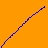
\includegraphics[width=\textwidth]{figs/fig_success_curves.png}
\caption{Planning success versus MPC replanning step, averaged over the conditions of each
shift family and all seeds. Top left: PushBlock shapes seen in training; top middle: held-out
shapes; top right: multiplicative visual corruptions (blur, salt-and-pepper, dark); bottom
left: colour shifts; bottom middle: PointMaze dynamics shifts; bottom right: held-out maze
layouts.}
\label{fig:curves}
\end{figure}

\begin{figure}[t]
\centering
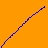
\includegraphics[width=\textwidth]{figs/fig_bars.png}
\caption{Final planning success per condition (mean $\pm$ s.d.\ over seeds).}
\label{fig:bars}
\end{figure}

\subsection{Ablations}

\begin{figure}[t]
\centering
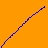
\includegraphics[width=0.95\textwidth]{figs/fig_adapt_stats.png}
\caption{Distribution of DTA-JEPA's online adaptation statistics across all conditions:
surprise, allocated gradient steps, learning-rate multiplier, number of updates and retrieved
memories. The allocation is strongly non-uniform, which is the mechanism the method claims.}
\label{fig:stats}
\end{figure}

\subsection{Uncertainty calibration and compute allocation}

\subsection{Continual (cross-episode) adaptation}

